%TODO: в конечной версии draft заменить final
\documentclass[oneside, final, 14pt, a4paper]{extreport}
\renewcommand{\rmdefault}{ftm} % Times New Roman

\usepackage[utf8]{inputenc}
\usepackage[russianb]{babel}
\usepackage{amssymb}
\usepackage{amsmath}
\usepackage[labelsep = period]{caption}
\usepackage{moreverb}

% flowcharts
\usepackage{tikz}
\usetikzlibrary{shapes,arrows,
	decorations.pathreplacing,decorations.pathmorphing}
	
% for tables
\usepackage{multirow}
\usepackage{hhline}

% include pictures
\usepackage{graphicx}
\DeclareGraphicsExtensions{.png}
\graphicspath{ {pics/} }

% красная строка для всех абзацев
\usepackage{indentfirst}

% отступы
\usepackage{vmargin}
\setmarginsrb{3cm}{2cm}{1.5cm}{2cm}{0pt}{0pt}{0pt}{1.3cm}

% полуторный интервал только для текста
\usepackage{setspace}
\onehalfspacing

% --------------------- определение команд рубрикации ---------------------
\newcommand\Chapter[1]
{
	\refstepcounter{chapter}
	\chapter*
	{
		\begin{huge}		
			\textbf
			{
				\raggedright \centering
				\chaptername\ \arabic{chapter}. #1\\
			}
		\end{huge}
		\bigskip
	}
	
	\addcontentsline{toc}{chapter}{\arabic{chapter}. #1}
}

\newcommand\Section[1]
{
	\refstepcounter{section}
	\section*
	{
		\raggedright \centering
		\arabic{chapter}. \arabic{section}. #1
	}
	
	\addcontentsline{toc}{section}{\arabic{chapter}. \arabic{section}. #1}
}

\newcommand\Subsection[1]
{
	\refstepcounter{subsection}
	\subsection*
	{
		\raggedright \centering
		\arabic{chapter}. \arabic{section}. \arabic{subsection}. #1		
	}
	
	\addcontentsline{toc}{subsection}{\arabic{chapter}. \arabic{section}.  \arabic{subsection}. #1}
}
% -------------------------------------------------------------------------

% точки в оглавлении
\usepackage{tocstyle}
\usetocstyle{allwithdot}

% точка вместо квадратных скобок в списке литературы
\makeatletter
\renewcommand*{\@biblabel}[1]{\hfill#1.}
\makeatother

%TODO: в конечной версии fussy заменить на sloppy
\sloppy

\begin{document}
\pagenumbering{gobble}

\renewcommand{\contentsname}{\centering Оглавление}
\tableofcontents
\thispagestyle{empty}

\chapter*{\centering Введение}
\addcontentsline{toc}{chapter}{Введение}

\pagenumbering{arabic}
\setcounter{page}{3}

\section*{\centering Актуальность}
\addcontentsline{toc}{section}{Актуальность}
Повсеместное внедрение компьютерных сетей, успехи в развитии оптоволоконных и беспроводных средств связи
споровождаются непрерывной сменой сетевых технологий, направленной на повышение быстродействия
и надёжности сетей. Однако создание опытного образца сети для оценки её эффективности не всегда является
оправданным с точки зрения времени и трудоёмкости, поэтому разработка математических моделей является актуальной задачей.

Для непрерывного количественного и качественного роста компьютерных сетей необходимо развитие фундаментальной
теории в этой области и создание инженерных методов анализа, направленных на сокращение сроков и повышение
качества проектирования компьютерных сетей.

В качестве такой теории выступает теория систем и сетей массового обслуживания.
Математические методы этой теории обеспечивают возможность решения многочисленных задач расчёта
характеристик качества функционирования различных компонентов компьютерных сетей.

\section*{\centering Цель}
\addcontentsline{toc}{section}{Цель}
В данной работе рассматривается анализ критериев времени и надёжности доставки информации в информационно-вычислительных
сетях (ИВС) с множественным методом доступа без коллизий,
построенных на основе технологий семейства Ethernet.

\section*{\centering Задачи}
\addcontentsline{toc}{section}{Задачи}
В задачи исследования входит:
\begin{enumerate}
	\item Изучение методики разработки моделей сетей.
	\item Разработка аналитических математических моделей ИВС.
	\item Разработка программы для вычисления стационарных и интегральных вероятностных характеристик заданной ИВС.
	\item Проведение модельного эксперимента.
\end{enumerate}

\section*{\centering Методы}
\addcontentsline{toc}{section}{Методы}
Модельный эксперимент и математические модели фрагментов сетей основываются на математическом аппарате и методах теории
систем и сетей массового обслуживания.

\section*{\centering Значимость}
\addcontentsline{toc}{section}{Значимость}
Разработанная программа должна автоматизировать рутинную работу по вычислению стационарных и интегральных вероятностных характеристик, плотностей распределения сообщений в маршрутах сети и среднего количества маршрутов между любыми двумя узлами сети.
%Она будет полезна при:
%\begin{itemize}
%	\item[-] предварительной оценке характеристик проектируемой ИВС
%	\item[-] оценке характеристик уже существующих ИВС
%	\item[-] изучении влияния изменений топологии и/или оборудования на характеристики ИВС
%\end{itemize}

\Chapter{Теоретичские основы разработки математической модели ИВС}
\Section{Однородные экспоненциальные сети}
Предметом изучения сетей массового обслуживания (СеМО) являются методы количественного анализа очередей при взаимодействии
множества центров обслуживания и потоков сообщений.

СеМО представляет собой совокупность конечного числа \( M \) обслуживающих центров, в которой циркулируют сообщения,
переходящие в соответствии с маршрутной матрицей (см. \ref{subsection:routingMatrix})  из одного центра сети в другой.
Центром обслуживания является система массового обслуживания, состоящая из \( A \; (1 \leqslant A \leqslant \infty) \) одинаковых приборов
и буфера объёмом \( C \; (0 \leqslant C \leqslant \infty) \). Если в момент поступления сообщения все обслуживающие приборы центра заняты, то сообщение занимает очередь в буфере и ожидает обслуживания \cite[стр. ~90]{vishnevsky}.

В дальнейшем будем полагать, что объём буфера в центре обслуживания \( C = \infty \), время обслуживания заявок распределено по экспоненциальному закону, а распределение входящего потока имеет распределение Пуассона.

СеМО с такими распределениями длительности обслуживания и входящего потока являются однородными экспоненциальными сетями
или сетями Джексона \cite[стр. ~94]{vishnevsky}. Такая модель даёт верхнюю границу оценки (худший вариант)
и стационарные вероятности состояний сети имеют мультипликативную форму.

В данной работе используются открытые сети Джексона, обрабатывающие \( F \) входящих потоков. В открытую сеть сообщения поступают из внешнего источника,
могут покидать сеть после завершения обслуживания и интенсивность входного потока не зависит от состояния сети.

\Subsection{Пуассоновский поток}
Предположение о том, что входящий поток является Пуассоновским, значительно облегчает математические выкладки при достаточной точности.

\noindent Пуассоновский поток имеет следующие свойства \cite[стр. ~12]{hinchin} \cite[стр. ~7]{pisarev}:
\begin{enumerate}
	\item Стационарность --- вероятность появления \( k \) событий на любом промежутке времени зависит только от числа \( k \) и от длительности
	\( t \) промежутка.
	
	\item Ординарность --- вероятность наступления за элементарный промежуток времени более одного события мала по сравнению с вероятностью
	наступления за этот промежуток не более одного события и ей можно пренебречь.
	
	\item Независимость --- вероятность появления \( k \) на любом промежутке времени не зависит от того, появлялись или не появлялись
	события в моменты времени, предшествующие началу рассматриваемого промежутка.
\end{enumerate}

\Subsection{Маршрутная матрица}
\label{subsection:routingMatrix}
Маршрутная матрица задаёт структуру соединений узлов сети (топологию) и вероятности переходов сообщения из одного центра сети, после завершения обслуживания
в нём, в другой.
Для открытой сети в качестве внешнего источника вводится новый центр с индексом \( 0 \).
Таким образом маршрутная матрица имеет вид \( P = \: \parallel P_{ij} \parallel \),
где \cite[стр. ~17]{klimanov:manual_stankin}:
\\ \( i, j = \overline{0, n}, \: n \) - число узлов в сети,
\\ \( P_{0j} \) - вероятность поступления сообщения в \( M_j \) узел сети из внешнего источника,
\\ \( P_{i0} \) - вероятность покидания сообщением сети после окончания обработки в \( M_i \) узле,
\\ \( P_{ \substack{ ij \\ i \neq j }} \) - вероятность перехода сообщения в узел \( M_j \) после обработки в \( M_i \).
\\ \( P_{00} = 0\).

\noindent В маршрутной матрице должно выполняться равенство \( \sum\limits_{j = 0}^{n} P_{ij} = 1, \: i = \overline{1, n} \).
Т.е. событие, состоящие в том, что сообщение после обработки в узле сети перейдёт в другой узел или покинет сеть --- достоверное.

Для сети, обрабатывающей \( F \) входящих потоков, необходимо задать \( F \) маршрутных матриц \( P^{m}, \: m = \overline{1, F} \) для каждого входного потока.

\Section{Методика разработки математической модели ИВС}
\label{section:mathmodel}
Одним из самых распространнёных методов для разработки аналитической математической модели ИВС является приближённая
декомпозиционная модель сети массового обслуживания, основанная на составлении уравнений баланса средних для класса мультипликативных сетей.
Эта модель допускает простую декомпозицию всей сети на отдельные элементы и обратную операцию - композицию. Такой подход позволяет проводить
анализ каждого фрагмента сети независимо, а затем объединять эти фрагменты, получая обобщённые характеристики.

Первый этап методики состоит в декомпозиции сети на отдельные фрагменты. В зависимости от уровня детализации выделяют 4 уровня декомпозиции \cite[стр. ~15]{klimanov:manual_stankin}:
\begin{enumerate}
	\item Состоит из набора функциональных элементов (терминалов, моноканалов, канальных станций), каждый из которых может быть представлен
	в виде отдельной СМО. Самый подробный уровень декомпозиции.	
	\item Учитывает особенности взаимодействия отдельных элементов 1-го \\ уровня в пределах всей ИВС.
	\item Учитывает взаимодействие нескольких ИВС элементарных топологий (физическая шина, физическое кольцо), связанных между собой в единую ИВС
	простой топологии (дерево, звезда, и т.д.).
	\item Учитывает взаимодействие любых ИВС 2-го и 3-го уровня, связанных в единую ИВС произвольной топологии.
\end{enumerate}
Декомпозиция позволяет преодолеть трудности анализа ИВС большой размерности за счёт разделения ИВС на иерархический набор более простых моделей \cite[стр. ~11]{klimanov:thesis}

Второй этап методики независимо от уровня декомпозиции заключается в разработке отдельных математических моделей всех составляющих на всех уровнях декомпозиции
и состоит из следующих подэтапов \cite[стр. ~16]{klimanov:manual_stankin}:
\begin{enumerate}
	\item  Составление уравнений баланса интенсивностей потоков.
	\item  Вычислеие коэффициентов передачи из уравнений баланса.
	\item  Вычисление стационарных вероятностно-временных характеристик \\ (ВВХ) для каждого отдельного элемента СеМО.
	\item  Вычисиление интегральных ВВХ при взаимодействии двух любых абонентов сети.
\end{enumerate}

Исходными параметрами модели являются интенсивности обслуживающих узлов сети \( \mu_{i}^{m} \), интенсивности поступления сообщений из внешнего источника
\( \lambda_{i}^{m} \) и маршрутная матрица \( P^{m} \) для каждого входного потока \( m = \overline{1, F} \).

\Subsection{Уравнения баланса}
\label{subsection:balanceEquations}
Уравнения баланса позволяют найти общие интенсивности потоков \( \lambda_{i}^{'m} \) сообщений в стационарном режиме открытой СеМО (стационарным режимом называется состояние сети,
при \( t \rightarrow \infty \) и \( \rho \leqslant 1 \) (см. \ref{subsection:coefficientOfLoading})).

\[ \lambda_{i}^{'m} = e_{i}^{m} \lambda_{0}^{m} \]
\( e_{i}^{m} \) - коэффициенты передачи, получаемые при решении уравнений баланса,
\( \lambda_{0}^{m} = \sum\limits_{i = 1}^{n} \lambda_{i}^{m}\) - суммарная интенсивность всех внешних потоков типа \( m \).

Общая интенсивность птоков складывается из интенсивностей поступления сообщений в \( M_{i} \) узел из внешнего источника \( P_{0i}^{m} \lambda_{0}^{m}, P_{0i}^{m} = \frac{\lambda_{j}^{m}}{\lambda_{0}^{m}} \)
и интенсивностей поступления сообщений от других узлов \( e_{j}^{m} P_{ji}^{m} \lambda_{0}^{m} \) \cite[стр. ~17]{klimanov:manual_stankin}.

\[ e_{i}^{m} \lambda_{0}^{m} = P_{0i}^{m} \lambda_{0}^{m} + \sum\limits_{j = 1}^{n} e_{j}^{m} P_{ji}^{m} \lambda_{0}^{m}, i = \overline{1, n}, m = \overline{1, F} \]

\noindent Видно, что можно сократить обе части уравнения на \( \lambda_{0}^{m} \).

\[ e_{i}^{m} = P_{0i}^{m} + \sum\limits_{j = 1}^{n} e_{j}^{m} P_{ji}^{m}, i = \overline{1, n}, m = \overline{1, F} \]

\[ \Updownarrow \]

\[
 	\left\{
		\begin{aligned}
			& e_{1}^{m} = P_{01}^{m} + e_{1}^{m} P_{11}^{m} + \cdots + e_{n}^{m} P_{n1}^{m} \\
			& \vdots \\
			& e_{n}^{m} = P_{0n}^{m} + e_{1}^{m} P_{1n}^{m} + \cdots + e_{n}^{m} P_{nn}^{m}
		\end{aligned}
	\right.
\]

\noindent После решения этой системы уравнений получаем \( e_{i}^{m} \) для каждого узла, что позволяет рассчитать \( \lambda_{i}^{'m} \).

\Subsection{Коэффициент загрузки}
\label{subsection:coefficientOfLoading}
Коэффициент загрузки для узла \( M_{i} \) вычисляется по формуле
\[ \rho_{i} = \sum\limits_{m = 0}^{F} \rho_{i}^{m}, \: \rho_{i}^{m} = \frac{\lambda_{i}^{'m}}{\mu_{i}^{m}}, \:
i = \overline{1, n} \]
\( \rho_{i}^{m} \)- коэффициент использования узла, характеризующий соотношение интенсивности входящего потока к интенивности обработки \cite[стр. ~34]{kleinrock:qs}. \\
Для существования стационарного распределения числа сообщений в системе необходимо выполнение условия
\[ 0 \leqslant \rho_{i}, \rho_{i}^{m} \leqslant 1, \: i = \overline{1, n} \]
что согласуется с интуитивными соображениями: для того, чтобы в системе не накапливалась бесконечная очередь, необходимо, чтобы в среднем сообщения в системе обслуживались быстрее, чем они туда поступают \cite[стр. ~35]{vishnevsky}.

\Subsection{Стационарные вероятностно-временные характеристики}
\label{subsection:sptc}
Для каждого узла  \( M_{i} \) сети определяются четыре вероятностно- \\ временные характеристики \cite[стр. ~19]{klimanov:manual_stankin}:
\begin{enumerate}
	\item Средняя длительность ожидания обслуживания.
	\[
		W_{i} = \frac{ \frac{1}{2} \sum\limits_{m = 0}^{F} \frac{ \rho_{i}^{m} (1 + V_{i}^{m^{2}}) }{ \mu_{i}^{m}} }{ 1 - \rho_{i} }
		= \Biggl\lvert \begin{aligned} & V_{i}^{m} = 1 \\ & \text{для распределения Пуассона} \end{aligned} \Biggr\rvert
		= \frac{ \sum\limits_{m = 0}^{F} \frac{ \rho_{i}^{m} }{ \mu_{i}^{m}} }{ 1 - \rho_{i} }
	\]
	\( V_{i}^{m} \) - коэффициент вариации времени обработки.
	
	\item Средняя длительность пребывания сообщения в узле для потока \( m \).
	\[ U_{i}^{m} = W_{i} + \frac{1}{\mu_{i}^{m}} \]
	\( \frac{1}{\mu_{i}^{m}} \) - время обработки сообщения.
	
	\item Средняя длина очереди сообщений в узле для потока \( m \).
	\[ L_{i}^{m} = \lambda_{i}^{'m} W_{i} \]
	
	\item Среднее число сообщений в узле для потока \( m \), хакатеризующее количество сообщений, находящихся в очереди на обработку,
	и количество сообщений, обрабатывающихся в узле.
	\[ N_{i}^{m} = \lambda_{i}^{'m} U_{i}^{m} \]
\end{enumerate}
Эти формулы справедливы для многих моделей СМО и называются формулами Литтла \cite[стр. ~37]{vishnevsky}.

\Subsection{Интегральные вероятностно-временные характеристики}
\label{subsection:iptc}
Для определения интегральных ВВХ используются стационарные ВВХ, полученные для каждого узла сети, и анализ маршрутов движения сообщений между двумя абнентами
\( A_{i} \) и \( A_{j}, \: i \neq j \).

Любой маршрут между двумя любыми абонентами принадлежит к одному из трёх типов \cite[стр. ~20]{klimanov:manual_stankin}:
\begin{enumerate}
	\item Последовательная обработка сообщений на конечном числе элементов сети.
	\begin{figure}[h!]
		\begin{center}
			\begin{picture}(200, 20)(-10, -10)
				\put(0, 0){\circle{20}}
				\put(-5, -3){\begin{scriptsize} 1 \end{scriptsize}}
	
				\put(10, 0){\vector(1, 0){20}}
				
				\put(40, 0){\circle{20}}
				\put(35, -3){\begin{scriptsize} 2 \end{scriptsize}}
		
				\put(50, 0){\vector(1, 0){20}}
				
				\put(78, -1){\( \dots \)}

				\put(102, 0){\vector(1, 0){20}}
				
				\put(132, 0){\circle{20}}
				\put(119.5, -3){\begin{scriptsize} \( n - 1 \)\end{scriptsize}}
				
				\put(142, 0){\vector(1, 0){20}}
				
				\put(172, 0){\circle{20}}
				\put(166.5, -2.5){\begin{scriptsize} \( n \)\end{scriptsize}}
			\end{picture}
		\end{center}

	\caption{Последовательная обработка}
	\label{pic:sequence}
	\end{figure}
	
	Маршрут состоит из последовательно соединённых узлов сети (рис. \ref{pic:sequence}). Интегральные характеристики маршрута вычисляются как сумма
	соответсвующих характеристик узлов, входящих в маршрут. \\
	Среднее время ожидания обслуживания в маршруте.
	\[ W = \sum\limits_{i = 1}^{n} W_{i} \]
	Среднее время пребывания требования в маршруте для потока \( m \).
	\[ U^{m} = \sum\limits_{i = 1}^{n} U_{i}^{m} \]
	Средняя длина очереди требований в маршруте для потока \( m \).
	\[ L^{m} = \sum\limits_{i = 1}^{n} L_{i}^{m} \]
	Среднее число требований в маршруте для потока \(	m \).
	\[ N^{m} = \sum\limits_{i= 1}^{n} N_{i}^{m} \]
	
	\item Параллельные варианты обработки с определёнными значениями вероятности выбора рассматриваемого варианта.
	\begin{figure}[h!]
		\begin{center}
			\begin{picture}(220, 120)
				\put(10, 50){\circle{20}}
				\put(5.5, 47){\begin{scriptsize} \( i \) \end{scriptsize}}
				
				\put(70, 100){\begin{scriptsize} \( \beta_{1} \) \end{scriptsize}}
				\put(20, 50){\vector(4, 3){80}}
				
				\put(110, 110){\circle{20}}
				\put(105, 107){\begin{scriptsize} 1 \end{scriptsize}}
				
				\put(120, 110){\vector(4, -3){80}}
				
				\put(70, 70){\begin{scriptsize} \( \beta_{2} \) \end{scriptsize}}
				\put(20, 50){\vector(4, 1){80}}
				
				\put(110, 70){\circle{20}}
				\put(105, 67){\begin{scriptsize} 2 \end{scriptsize}}
				
				\put(120, 70){\vector(4, -1){80}}
				
				\put(20, 50){\vector(4, -1){80}}				
				\put(108, 35){\( \vdots \)}
				
				\put(70, 25){\begin{scriptsize} \( \beta_{l} \) \end{scriptsize}}
				\put(20, 50){\vector(2, -1){80}}
				
				\put(110, 10){\circle{20}}
				\put(105.5, 7){\begin{scriptsize} \( l \) \end{scriptsize}}
				
				\put(120, 10){\vector(2, 1){80}}
				
				\put(210, 50){\circle{20}}
				\put(205.5, 47){\begin{scriptsize} \( j \) \end{scriptsize}}
			\end{picture}
		\end{center}

	\caption{Параллельные варианты}
	\label{pic:parallel}
	\end{figure}
	
	Маршрут зависит от одного из выбранного параллельного варианта (рис. \ref{pic:parallel}). Заданы параллельные варианты обработки с вероятностями выбора
	(см. \ref{subsection:pathsProbabilities}) \( \beta_{k}, \: k = \overline{1, l}, \: l \) - количество альтернатив и должно выполняться нормирующее условие
	\( \sum\limits_{k = 1}^{l} \beta_{k} = 1 \).
	
	Интегральные ВВХ определяются следующим образом. \\
	Среднее время ожидания обслуживания в маршруте.
	\[ W = W_{i} + \sum\limits_{k = 1}^{l} \beta_{k} W_{k} + W_{j} \]
	Среднее время пребывания требования в маршруте для потока \( m \).
	\[ U^{m} = U_{i}^{m} + \sum\limits_{k = 1}^{l} \beta_{k} U_{k}^{m} + U_{j}^{m} \]
	Средняя длина очереди требований в маршруте для потока \( m \).
	\[ L^{m} = L_{i}^{m} + \sum\limits_{k = 1}^{l} \beta_{k} L_{k}^{m} + L_{j}^{m} \]
	Среднее число требований в маршруте для потока \( m \).
	\[ N^{m} = N_{i}^{m} + \sum\limits_{k = 1}^{l} \beta_{k} N_{k}^{m} + N_{j}^{m} \]
	
	\item Комбинация первых двух типов.
	\begin{figure}[h!]
		\begin{center}
			\begin{picture}(382, 120)
				\put(10, 50){\circle{20}}
				\put(5.5, 47){\begin{scriptsize} \( i \) \end{scriptsize}}
				
				\put(70, 100){\begin{scriptsize} \( \beta_{1} \) \end{scriptsize}}
				\put(20, 50){\vector(4, 3){80}}
				
				%--------------------------------------------------------------------------
					\put(110, 110){\circle{20}}
					\put(105, 107){\begin{scriptsize} 1 \end{scriptsize}}
	
					\put(120, 110){\vector(1, 0){15}}
				
					\put(145, 110){\circle{20}}
					\put(140, 107){\begin{scriptsize} 2 \end{scriptsize}}
		
					\put(155, 110){\vector(1, 0){15}}

					\put(183, 109){\( \dots \)}

					\put(207, 110){\vector(1, 0){15}}
				
					\put(237, 110){\circle{20}}
					\put(224.5, 107){\begin{scriptsize} \( n - 1 \)\end{scriptsize}}
					
					\put(247, 110){\vector(1, 0){15}}
				
					\put(272, 110){\circle{20}}
					\put(266.5, 107.5){\begin{scriptsize} \( n \)\end{scriptsize}}	
				%--------------------------------------------------------------------------
				
				\put(282, 110){\vector(4, -3){80}}
				
				\put(70, 70){\begin{scriptsize} \( \beta_{2} \) \end{scriptsize}}
				\put(20, 50){\vector(4, 1){80}}
				
				%--------------------------------------------------------------------------					
					\put(110, 70){\circle{20}}
					\put(105, 67){\begin{scriptsize} 1 \end{scriptsize}}
	
					\put(120, 70){\vector(1, 0){15}}
				
					\put(145, 70){\circle{20}}
					\put(140, 67){\begin{scriptsize} 2 \end{scriptsize}}
		
					\put(155, 70){\vector(1, 0){15}}

					\put(183, 69){\( \dots \)}

					\put(207, 70){\vector(1, 0){15}}
				
					\put(237, 70){\circle{20}}
					\put(224.5, 67){\begin{scriptsize} \( n - 1 \)\end{scriptsize}}
					
					\put(247, 70){\vector(1, 0){15}}
				
					\put(272, 70){\circle{20}}
					\put(266.5, 67.5){\begin{scriptsize} \( n \)\end{scriptsize}}					
				%--------------------------------------------------------------------------
				
				\put(282, 70){\vector(4, -1){80}}
				
				\put(20, 50){\vector(4, -1){80}}				
				\put(108, 35){\( \vdots \)}
				
				\put(70, 25){\begin{scriptsize} \( \beta_{l} \) \end{scriptsize}}
				\put(20, 50){\vector(2, -1){80}}
				
				%--------------------------------------------------------------------------					
					\put(110, 10){\circle{20}}
					\put(105, 7){\begin{scriptsize} 1 \end{scriptsize}}
	
					\put(120, 10){\vector(1, 0){15}}
				
					\put(145, 10){\circle{20}}
					\put(140, 7){\begin{scriptsize} 2 \end{scriptsize}}
		
					\put(155, 10){\vector(1, 0){15}}

					\put(183, 9){\( \dots \)}

					\put(207, 10){\vector(1, 0){15}}
				
					\put(237, 10){\circle{20}}
					\put(224.5, 7){\begin{scriptsize} \( n - 1 \)\end{scriptsize}}
					
					\put(247, 10){\vector(1, 0){15}}
				
					\put(272, 10){\circle{20}}
					\put(266.5, 7.5){\begin{scriptsize} \( n \)\end{scriptsize}}					
				%--------------------------------------------------------------------------
				
				\put(282, 10){\vector(2, 1){80}}
				
				\put(372, 50){\circle{20}}
				\put(367.5, 47){\begin{scriptsize} \( j \) \end{scriptsize}}
			\end{picture}
		\end{center}

	\caption{Комбинированный тип обработки}
	\label{pic:combine}
	\end{figure}	
	
	Маршрут зависит от одного из выбранных параллельных маршрутов (рис. \ref{pic:combine}).
	
	Комбинированный тип обработки включает в себя рассмотрение \\ сложных альтернатив, представляющих собой конечную комбинацию двух предыдущих
	топологических типов.
	
	Интегральные ВВХ в этом случае определяются как в предыдущем случае, но вместо альтернативных вариантов рассматриваются альтернативные маршруты. \\
	Среднее время ожидания обслуживания в маршруте.
	\[ W = W_{i} + \sum\limits_{k = 1}^{l} \left( \beta_{k} \sum\limits_{x = 1}^{n} W_{x} \right) + W_{j} \]
	Среднее время пребывания требования в маршруте для потока \( m \).
	\[ U^{m} = U_{i}^{m} + \sum\limits_{k = 1}^{l} \left( \beta_{k} \sum\limits_{x = 1}^{n} U_{x}^{m} \right) + U_{j}^{m} \]	
	Средняя длина очереди требований в маршруте для потока \( m \).
	\[ L^{m} = L_{i}^{m} + \sum\limits_{k = 1}^{l} \left( \beta_{k} \sum\limits_{x = 1}^{n} L_{x}^{m} \right) + L_{j}^{m} \]	
	Среднее число требований в маршруте для потока \( m \).
	\[ N^{m} = N_{i}^{m} + \sum\limits_{k = 1}^{l} \left( \beta_{k} \sum\limits_{x = 1}^{n} N_{x}^{m} \right) + N_{j}^{m} \]		
\end{enumerate}

\Subsection{Вероятность выбора маршрута}
\label{subsection:pathsProbabilities}
Для вычисления интегральных ВВХ необходимо определить вероятности выбора альтернативных маршрутов (см. \ref{subsection:iptc}).

Для этого нужно учитывать вероятности перехода между узлами, заданные маршрутной матрицей \( P^{m} \) (см. \ref{subsection:routingMatrix}), и нормирующее условие
\[ \sum\limits_{k = 1}^{l} \beta_{k} = 1 \]
указывающее, один из маршрутов будет обязательно выбран.

Вероятность выбора маршрута определяется отношением произведения вероятностей перехода требований из узла \( M_{ R_{j}^{i} } \) в узел \( M_{ R_{j+1}^{i} } \)
\( i \) - го маршрута к сумме произведений вероятностей переходов требований всех альтернативных маршрутов (нормировочной величине).
\enlargethispage{\baselineskip}
\[ \beta_{i} = \frac{ \prod\limits_{j} P_{ R_{j}^{i}, R_{j + 1}^{i} } }{S} \]
\( S = \sum\limits_{i} \left( \prod\limits_{j} P_{ R_{j}^{i}, R_{j+1}^{i} } \right) \) - нормировочная величина. \\
\( R^{i} \) - совокупность узлов, составляющих альтернативный маршрут  \( i \). \\
\( P_{ R_{j}^{i}, R_{j+1}^{i} } \) - вероятность перехода между узлами, задаваемая маршрутной матрицей.

\Subsection{Плотность распределения количества сообщений в маршруте}
Плотность распределения количества сообщений для произвольного \\ маршрута определяется следующим способом:
\[ g_{i} (t) = \sum\limits_{i = 1}^{n} H_{i} (\mu_{i} - \lambda_{i}^{'}) e^{ -(\mu_{i} - \lambda_{i}^{'}) t } \]
\[ H_{i} = \prod\limits_{ \substack{ j = 1 \\ j \neq i } }^{n} \frac{ \mu_{j} - \lambda_{j}^{'} }{ \mu_{j} - \lambda_{j}^{'} - \mu_{i} - \lambda_{i}^{'} } \]
где \( n \) - количество узлов в маршруте.

\Section{Определение интенсивностей обслуживающих приборов, работающих на основе технологий семейства Ethernet}
\label{section:ethernet}
Для определения интенсивности обслуживания \( \mu \), которая характеризует максимальное количество кадров в секунду
\footnote{При указании производительности сетей термины "кадр" и "сообщение" обычно используются как синонимы. Следовательно единицы измерения производительности кадр/с и сообщение/с являются аналогичными. \cite{klimanov:manual_mpei}}
, обрабатываемых обслуживающим прибором, рассмотрим кадр формата Ethernet Version 2, т.к. на практике в оборудовании Ethernet используется только он \cite[стр. ~361]{olifers}.

Стандарт Ethernet определяет длину служебных полей кадра и преамбулу по 18 и 8 байт соответственно. От сюда следует что длина кадра в битах равна \( 8 * (X + 26), \: X \) - длина поля данных. Поле данных может иметь длину от 46 до 1500 байт \cite[стр. ~361]{olifers}. Таким образом минимальная длина кадра равна \( 46 + 26 = 72 \) байта, а максимальная 1526 байт.

Время передачи битов кадра определяется битовыми интервалами \( bt = \frac{1}{S}, \: S \) - битовая скорость.
Для передачи кадра длиной \( X \) потребуется время равное \( 8 * (X + 26) * bt \). Прибавив межкадровый интервал \( IFG = 96 * bt \) получим
период следования кадров с длиной поля данных \( X \).
\[ T = 8 * (X + 26) * bt + IFG \]

Итенсивность обслуживания \( \mu \), которая характеризует максимальное количество кадров в секунду, обрабатываемых обслуживающим прибором, есть величина обратно пропорциональная периоду \( T \).
\[ \mu = \frac{1}{T} = \frac{1}{ 8 * (X + 26) * bt + IFG } \]

Проведя не сложные расчёты можно получить интенсивности обслуживания для пакетов различной длины с учётом выбранной технологии передачи данных (табл. \ref{tab:mu}).

\begin{table}[h!]
	\begin{tabular}{|p{0.22\textwidth}|p{0.22\textwidth}|p{0.22\textwidth}|p{0.22\textwidth}|}
	\hline Технология Ethernet & Битовая скорость & Длина кадра (байт) & Интенсивность \( \mu \) (кадр/мс) \\
	\hline \multirow{2}{*}{Fast Ethernet} 	& \multirow{2}{*}{100 Мбит/с} 	& 72 	& 148.800 \\
	\hhline{~~--}				  			& \multirow{2}{*}{}           	& 1526 	& 8.127 \\ 
	
	\hline \multirow{2}{*}{Gigabit Ethernet} 	& \multirow{2}{*}{1 Гбит/с} 		& 72 	& 1488.095 \\
	\hhline{~~--}				  			& \multirow{2}{*}{}           	& 1526 	& 81.274 \\ 
	
	\hline \multirow{2}{*}{10G Ethernet} 		& \multirow{2}{*}{10 Гбит/с} 	& 72 	& 14880.952 \\
	\hhline{~~--}				  			& \multirow{2}{*}{}           	& 1526 	& 812.744 \\ 
	
	\hline \multirow{2}{*}{40G Ethernet} 		& \multirow{2}{*}{40 Гбит/с} 	& 72 	& 59523.800 \\
	\hhline{~~--}				  			& \multirow{2}{*}{}           	& 1526 	& 3250.975 \\ 
	
	\hline \multirow{2}{*}{100G Ethernet} 	& \multirow{2}{*}{100 Гбит/с} 	& 72 	& 148809.524 \\
	\hhline{~~--}				  			& \multirow{2}{*}{}           	& 1526 	& 8127.438 \\
	\hline
	\end{tabular}

	\caption{Интенсивности обслуживания для пакетов различной длины с учётом выбранной технологии передачи данных}
	\label{tab:mu}
\end{table}

\Section{Структурная надёжность сетей}
Надёжность какого-либо объекта -- свойство, заключающееся в способности выполнять поставленные задачи в определённых условиях эксплуатации.
Состояние объекта, при котором он способен выполнять заданные функции, сохраняя значения основных параметров в пределах, установленных нормативно-технической документацией, называют работоспособностью, а состояние, в котором объект удовлетворяет указанным требованиям, -- его исправностью.
Событие, заключающееся в нарушении работоспособности объекта, называют отказом.

Для информационых сетей, являющихся сложными системами, состоящими из элементов разнородных по своим свойствам, показателям надёжности, назначению, дате изготовления, сроку ввода в эксплуатацию и т.п., выделяют два основных аспекта надёжности \cite{reliability}:
\begin{enumerate}
	\item Аппаратурный. Под ним понимают проблему надёжности отдельных элементов, входящих в узлы и линии сети.
	\item Структурный. Связан с возможностью существования в сети путей доставки информации.
\end{enumerate}

В данной работе рассматривается структурная надёжность, определяемая средним количеством маршрутов маршрутов между двумя произвольными вершинами сети.
Эта характеристика вполне хорошо отражает структурную надёжность сети, т.к. чем больше альтернативных маршрутов существует между любыми двумя узлами сети, тем при большем количестве неисправных участков сети она будет оставаться работоспособной и способной передачать сообщени между любыми двумя узлами.
Более строгие модели надёжности сетей будут рассмотрены в магистерской диссертации.

\Chapter{Программная реализация}
\Section{Постановка задачи}
Программа должна удовлетворять следующим требованиям:
\begin{enumerate}
    \item Вычислять стационарные и интегральные ВВХ для заданной пользователем модели ИВС.
    \item Проверять корректность введённой пользователем модели ИВС.
    \item При невозможности вычисления каких-либо характеристик сообщать об этом пользователю.
\end{enumerate}

Программа будет выполнена в виде консольного приложения, т.к. этого достаточно для поставленной задачи и позволяет сконцентрироваться на реализации и достижении поставленных требований. Также это позволит программе без проблем запускаться на различных операционны системах.

\Section{Программная платформа}
Выбрана программная платформа Mono --- кроссплатформенная реализация Microsoft .Net Framework с открытым исходным кодом.
Mono поддерживает Windows, Linux, BSD, Mac OS X и другие операционные системы и множетсво процессорных платформ, что
позволяет писать переносимые приложения на C\#.
Среда разработки --- MonoDevelop.

\Section{Описание модели ИВС}
Модель ИВС одонозначно задаётся интенсивностями обслуживания \( \mu_{i}^{m} \), интенсивностями поступления сообщений
\( \lambda_{i}^{m} \) и маршрутной матрицей \( P^{m} \) для каждого входного потока \( m = \overline{1, F} \)
(см. \ref{section:mathmodel}). Таким образом надо решить как пользователь будет передавать программе описание модели ИВС.

Для этой цели используется XML файл, в котором задаются параметры модели. XML имеет простой синтаксис, удобный как для составления и чтения файлов человеком, так и для машинной обработки и генерации.

\begin{figure}[h!]
    \begin{listing}{1}
<NetworkConfiguration Name="Linear topology">
  <RoutingMatrix>
	<Row>0; -;  -;  -;  -</Row>
	<Row>0.25;  0;  0.75;   0;  0</Row>
	<Row>0.25;  0.375;  0;  0.375;  0</Row>
	<Row>0.25;  0;  0.375;  0;  0.375</Row>
	<Row>0.25;  0;  0;  0.75;   0</Row>
  </RoutingMatrix>
        
  <Nodes Count="4">
	<Lambda>17; 14; 13; 16</Lambda>
		        
	<Mu>
	  <Ethernet Type="Gigabit" FrameLength="Max"/>
	</Mu>
  </Nodes>
</NetworkConfiguration>\end{listing}
    
    \caption{Описание ИВС линейной топологии из 4-х узлов и одним потоком}
    \label{pic:xml}
\end{figure}

\begin{figure}[h!]
	\begin{center}
		\begin{picture}(200, 40)(-10, -10)
			\put(0, 0){\circle{30}}
			\put(-10, -3){ \( \mu_{1} \) }
			
			\put(-30, 45){\vector(1, -1){29}}	
			\put(-1, 16){\vector(-1, 1){29}}
			\put(-15, 30){ \( \lambda_{1} \)}			
			\put(16, 0){\vector(1, 0){28}}
			\put(44, 0){\vector(-1, 0){28}}
				
			\put(60, 0){\circle{30}}
			\put(50, -3){ \( \mu_{2} \) }
			
			\put(30, 45){\vector(1, -1){29}}
			\put(59, 16){\vector(-1, 1){29}}
			\put(45, 30){ \( \lambda_{2} \) }
			\put(76, 0){\vector(1, 0){28}}
			\put(104, 0){\vector(-1, 0){28}}
				
			\put(120, 0){\circle{30}}
			\put(110, -3){ \( \mu_{3} \) }
			
			\put(90, 45){\vector(1, -1){29}}
			\put(119, 16){\vector(-1, 1){29}}
			\put(105, 30){ \( \lambda_{3} \) }
			\put(136, 0){\vector(1, 0){28}}
			\put(164, 0){\vector(-1, 0){28}}
				
			\put(180, 0){\circle{30}}
			\put(170, -3){ \( \mu_{4} \) }
			
			\put(150, 45){\vector(1, -1){29}}
			\put(179, 16){\vector(-1, 1){29}}
			\put(165, 30){ \( \lambda_{4} \) }
		\end{picture}
	\end{center}

	\caption{Сеть из 4-х узлов с линейной топологией}
	\label{pic:linear_demo}
\end{figure}

На рис. \ref{pic:xml} показан XML файл, задайющий модель ИВС, состоящей из 4-х узлов с линейной топологией и единственным потоком (рис. \ref{pic:linear_demo}).

При задании интенсивностей обслуживания (рис. \ref{pic:linear_demo}, строка 14) атрибут \verb:Type: обязателен и задаёт технологию Ethernet. Возможные значения этого атрибута Fast, Gigabit, \_10G, \_40G, \_100G. Атрибут \verb:FrameLength: задаёт длину используемых кадров. Его значение может быть  Min, Max, что соответствует минимальной (72) или максимальной (1526) длине кадра в байтах, или любое целое число от 72 до 1526.

Интенсивности поступления сообщений из внешнего источника здаются через точку с запятой для каждого узла сети, либо одним целым числом, если интенсивность для всех узлов одна, любо в процентах от интенсивности обслуживания, определённой в элементе \verb:Mu:.

Если в сети несколько потоков, то элементы \verb:Lambda: и \verb:Mu: задаются для каждого потока отдельно внутри элементов \verb:Stream: с атрибутом \verb:Index: (индексация с 0), указывающим к какому потоку относятся интенсивности (пример на рис. \ref{pic:demo4_config}).

В данном случае интенсивность обслуживания \( \mu \)  задаётся для пакетов максимальной длины технологии Gigabit Ethernet (см. \ref{section:ethernet}), интенсивность поступления сообщений \( \lambda \) задаётся в явном виде для каждого узла сети (пакеты/мс).
\[ \mu = (81.274, 81.274, 81.274, 81.274), \: \lambda = (17, 14, 13, 16) \]

Со 2-й по 8-ю строки задаётся маршрутная матрица.
\[ P = \left(\begin{matrix}
                0 & - & - & - & - \\
                0.25 & 0 & 0.75 & 0 & 0 \\
                0.25 & 0.375 & 0 & 0.375 & 0 \\
                0.25 & 0 & 0.375 & 0 & 0.375 \\
                0.25 & 0 & 0 & 0.75 & 0 \\
            \end{matrix}\right) \]
Маршрутная матрица это квадратная матрица с размерностью \( (n + 1 \times n + 1), n \) - количество узлов сети. Один дополнительный узел это внешний источник.

\noindent Маршрутная матрица должна обладать следующими свойствами:
\begin{enumerate}
	\item на главной диагонали должны быть нули
	\item сумма каждой строки должна быть равна 1
\end{enumerate}
Это гарантирует, что сообщение после обработки в узле его покинет.

Прочерки в строках задаваемой матрицы указывают программе, что надо вычислить соответствующие вероятности. Прочерки в первой строке указывают на необходимость вычисления вероятностей поступления сообщений из внешнего источника. Если прочерки есть и в других строках, то в соответствии со свойством 2 алгоритм присвоит пропускам значение
\[ \frac{ 1 - \text{сумма элементов строки} }{ \text{количество пропусков} } \]

В данном случае будут вычисляться только вероятности поступления сообщений из внешнего источника.
            
Парсинг (разбор) XML файла осуществляется с помощью стандартных средств языка C\# из пространств имён System.Xml и System.Xml.Linq.

\Section{Аргументы командной строки}
При вызове программе передаются несколько обязательных аргументов и один опциональный.

Обязательные аргументы \verb:netconfig:, \verb:startnode: и \verb:targetnode: задают путь к конфигурационному файлу, индексы начального и конечного узлов (индексация с 0) соответственно.

Необязательный аргумент \verb:log: обозначает необходмость создать лог, в который будет выведена вся информация, если вычисления закончились успешно, \verb:console: задаёт необходимость вывода информации в консоль, а \verb:matrix: указывает, надо ли выводить маршрутную матрицу. Аргумент \verb:matrix: полезен, когда маршрутная матрица имеет большую размерность и не корректно отображается при выводе.

Аргументы могут идти в любом порядке. Если обязательный аргумент пропущен, то произойдёт исключение и в консоли появится текст ошибки и какой аргумент пропущен.

\Section{Алгоритм работы программы}
% -------------------------------------------- flowcharts --------------------------------------------
% Define block styles
\tikzstyle{decision} = [diamond, draw, fill=white, 
    text width=6em, text badly centered, node distance=3cm, inner sep=0pt]
\tikzstyle{sqr_block} = [rectangle, draw, fill=white, 
    text width=5em, text centered, rounded corners, minimum height=4em]
\tikzstyle{rec_block} = [rectangle, draw, fill=white,
	text width=10em, text centered, rounded corners, minimum height=2em]
\tikzstyle{line} = [draw, -latex']
\tikzstyle{cloud} = [draw, ellipse,fill=white, node distance=3cm,
    minimum height=2em]
    
\begin{figure}[h!]
	\centering
	\begin{tikzpicture}[node distance = 2cm, auto]
	    % nodes
    		\node [rec_block] (parse) { парсинг аргументов командной строки };
	    \node [decision, below of=parse, node distance=3.5cm] (log) { нужно создавать лог? };
	    \node [sqr_block, left of=log, node distance=4.5cm] (create_log) { создание файла для лога };
	    \node [rec_block, below of=log, node distance=3.5cm] (parse_config) { парсинг конфигурационного файла };
    	    \node [rec_block, below of=parse_config, node distance=2.3cm] (compute_model) { расчёт параметров модели (рис. \ref{pic:flowchart_computeModel}) };
    	    \node [decision, below of=compute_model, node distance=3.8cm] (error) { исключения при расчёте параметров? };
    	    \node [rec_block, left of=error, node distance=6.5cm] (compute_stop) { завершение вычислений };
    	    \node [rec_block, below of=compute_stop, node distance=3cm] (error_output) { вывод в консоль сообщения об ошибке, в каком месте она возникла и стэк вызовов };
    	    \node [rec_block, below of=error, node distance=3.8cm] (output) {вывод данных на консоль и, если нужно, в лог};
    	    \node [rec_block, below of=output, node distance=2.4cm] (plotting) {построение графиков плотностей (рис. \ref{pic:flowchart_graphs}) };
    		% edges
    		\path [line] (parse) -- (log);
    		\path [line] (log) -- node [near start] {да} (create_log);
    		\path [line] (log) -- node [near start] {нет} (parse_config);
    		\path [line] (create_log) |- (parse_config);
    		\path [line] (parse_config) -- (compute_model);
    		\path [line] (compute_model) -- (error);
   		\path [line] (error) -- node [near start] {да} (compute_stop);
    		\path [line] (compute_stop) -- (error_output);
   		\path [line] (error) -- node [near start] {нет} (output);
    		\path [line] (output) -- (plotting);
	\end{tikzpicture}
	
	\caption{Общая блок-схема программной реализации}
	\label{pic:flowchart_common}
\end{figure}

\begin{figure}
	\centering
	\begin{tikzpicture}[node distance = 2cm, auto]
		% nodes
		\node [rec_block] (set_stream) { установка переменной \verb:stream: значения 0 };
		\node [decision, below of=set_stream, node distance=3.5cm] (stream) {\verb:stream: < числа потоков?};
		\node [rec_block, right of=stream, node distance=5.6cm] (compute_lambda0) { вычисление уммарной интенсивности внешних источников \( \lambda_{0} \)};
		\node [rec_block, below of=compute_lambda0, node distance=3cm] (compute_input) { вычисление  входящих интенсивностей для каждого узла сети };
		\node [rec_block, below of=compute_input, node distance=3.3cm] (compute_lambdaBar) { вычисление стационарных интенсивностей потоков \( \lambda^{'} \) для каждого узла сети };
		\node [rec_block, below of=compute_lambdaBar, node distance=3.3cm] (compute_rhoBar) { вычисление коэффициентов использования \( \rho^{'} \) для каждого узла сети };
		\node [rec_block, below of=compute_rhoBar, node distance=3cm] (compute_rho) { вычисление коэффициентов загрузки \( \rho \) для каждого узла сети };
		\node[rec_block,below of=compute_rho, node distance=2.8cm] (increment_stream) {увеличение переменной \verb:stream: на 1 };
		
		\node [rec_block, left of=stream, node distance=5.6cm] (find_paths) { \verb:FindPaths(): (\ref{subsection:findPaths}, рис. \ref{pic:function_findPaths}) };
		\node [rec_block, below of=find_paths] (compute_sptc) { вычисление стационарных ВВХ (\ref{subsection:compute_sptc}, рис. \ref{pic:function_computeSPTC}) };
		\node [rec_block, below of=compute_sptc] (compute_iptc) { вычисление интегральных ВВХ (\ref{subsection:compute_iptc}, рис. \ref{pic:flowchart_iptc}) };
		% edges
		\path [line] (set_stream) -- (stream);
		\path [line] (stream) -- node [near start] {да} (compute_lambda0);
		\path [line] (stream) -- node [near start] {нет} (find_paths);
		\path [line] (compute_lambda0) -- (compute_input);
		\path [line] (compute_input) -- (compute_lambdaBar);
		\path [line] (compute_lambdaBar) -- (compute_rhoBar);
		\path [line] (compute_rhoBar) -- (compute_rho);
		\path [line] (compute_rho) -- (increment_stream);
		\path [line] (increment_stream) -| (stream);
		\path [line] (find_paths) -- (compute_sptc);
		\path [line] (compute_sptc) -- (compute_iptc);
	\end{tikzpicture}
	
	\caption{Рассчёт параметров модели}
	\label{pic:flowchart_computeModel}
\end{figure}

\begin{figure}
	\centering
	\begin{tikzpicture}[node distance = 2cm, auto]
		% nodes
		\node [rec_block] (find_paths) { поиск всех путей между двумя заданными узлами (рис. \ref{pic:flowchart_paths}, \ref{pic:function_getPathsBetween}) };
		\node [rec_block, below of=find_paths, node distance=3cm] (compute_pathsProb) { вычисление вероятностей выбора для найденных маршрутов (рис. \ref{pic:function_computeTransitionProbabilities}) };
		\node [rec_block, below of=compute_pathsProb, node distance=3cm] (compute_iptc) { вычисление интегральных ВВХ для каждого потока };
		% edges
		\path [line] (find_paths) -- (compute_pathsProb);
		\path [line] (compute_pathsProb) -- (compute_iptc);
	\end{tikzpicture}
	
	\caption{Рассчёт интегральных ВВХ}
	\label{pic:flowchart_iptc}
\end{figure}

\begin{figure}
	\centering
	\begin{tikzpicture}[node distance = 2cm, auto]
		% nodes
		\node [rec_block] (find_paths) { самый короткий и самый длиный пути в сети };
		\node [decision, below of=find_paths, node distance=3cm] (equals) { они равны? };
		\node [sqr_block, left of=equals, node distance=5.5cm] (yes) { остаётся любой из путей };
		\node [sqr_block, right of=equals, node distance=5.5cm] (no) { остаются оба пути };
		\node [rec_block, below of=equals, node distance=3.5cm] (compute_density) { вычисление плотностей распределения сообщений в маршрутах };
		\node [rec_block, below of=compute_density, node distance=2.5cm] (create_plot) { создание графика };
		\node [rec_block, below of=create_plot] (show_plot) { вывод графика на экран };
		% edges
		\path [line] (find_paths) -- (equals);
   		\path [line] (equals) -- node [near start] {да} (yes);
   		\path [line] (equals) -- node [near start] {нет} (no);
   		\path [line] (yes) |- (compute_density);
  		\path [line] (no) |- (compute_density);  		
  		\path [line] (compute_density) -- (create_plot);
		\path [line] (create_plot) -- (show_plot);
	\end{tikzpicture}
	
	\caption{Построение графиков плотностей}
	\label{pic:flowchart_graphs}
\end{figure}

\begin{figure}
	\centering
	\begin{tikzpicture}[node distance = 2cm, auto]
		% nodes
		\node [decision] (paths) { начальный и конечный узлы равны? };
		\node [rec_block, right of=paths, node distance=5.5cm] (error) { выброс исключения };
		\node [rec_block, below of=paths, node distance=3.5cm] (exclude_loops) { удаляем связи начальной вершины со всеми остальными } ;
		\node [rec_block, below of=exclude_loops, node distance=2.6cm] (set_node) { установка переменной \verb:node: (промежуточный узел) значения 0 };
		\node [decision, below of=set_node, node distance=3.8cm] (node) {\verb:node: < числа узлов сети?};
		\node [rec_block, right of=node, node distance=5.2cm] (node_no) { возвращение списка найденных путей };
		\node [decision, below of=node, node distance=5.2cm] (link) { связь между \verb:node: и начальным узлом? };
		\node [rec_block, below of=link, node distance=3.7cm] (link_no) { переход на следующую итерацию };
		\node [decision, right of=link, node distance=5.3cm] (end) { \verb:node: = конечному узлу? };
		\node [rec_block, below of=end, node distance=3.6cm] (end_yes) { сохранение пути };
		\node [decision, right of=end, node distance=5.3cm] (exists) { кол-во овзвращённых путей  > 0? };
		\node [rec_block, above of=exists, node distance=4cm] (end_no) { рекурсивный вызов этой функции для промежуточного узла };
		\node [rec_block, below of=exists, node distance=3.7cm] (add) { сохранение найденных путей };
		% edges
		\path [line] (paths) -- node [near start] {нет} (exclude_loops);
		\path [line] (paths) -- node [near start] {да} (error);
		\path [line] (exclude_loops) -- (set_node);
		\path [line] (set_node) -- (node);
		\path [line] (node) -- node [near start] {нет} (node_no);
		\path [line] (node) -- node [near start] {да} (link);
		\path [line] (link) -- node [near start] {нет} (link_no);
		\path [line] (link) -- node [near start] {да} (end);
		\path [line] (end) |- node [near start] {нет} (end_no);
		\path [line] (end) -- node [near start] {да} (end_yes);
		\path [line] (end_no) -- (exists);
		\path [line] (exists) -- node [near start] {да} (add);
	\end{tikzpicture}
	
	\caption{Поиск всех путей между двумя узлами сети}
	\label{pic:flowchart_paths}
\end{figure}
% ----------------------------------------------------------------------------------------------------

\Section{Основные моменты реализации}
\Subsection{Функция расчёта параметров модели}
Функция \verb:ComputeParameters(): (рис. \ref{pic:function_computeParameters}) основная функция, которая после парсинга конфигурационного файла высчитывает следующие параметры:
\begin{itemize}
	\item[-] суммарная интенсивность внешних потоков \( \lambda_{0}^{m} \) (рис. \ref{pic:function_computeParameters}, строка 4)	
	\item[-] вероятности поступления сообщений из внешнего источника \( P_{0,j}^{m} \) \\ (рис. \ref{pic:function_computeParameters}, строка 11)
	\item[-] коэффициенты передачи \( e_{i}^{m} \) (рис. \ref{pic:function_computeParameters}, строка 14)
	\item[-] общие интенсивности потоков \( \lambda_{i}^{'m} \) (рис. \ref{pic:function_computeParameters}, строка 17)
	\item[-] коэффициенты использования узлов \( \rho_{i}^{m} \) и коэффициенты загрузки \( \rho_{i} \) (рис. \ref{pic:function_computeParameters}, строка 20)
	\item[-] поиск всех путей между двумя заданными узлами, поис минимального и максимального путей в сети, поиск среднего числа путей между любыми двумя узлами сети (рис. \ref{pic:function_computeParameters}, строка 33).
\end{itemize}
Эти параметры дают достаточно инормации для дальнейших вычислений стационарных и интергральных ВВХ и плотностей распределения сообщений в маршрутах.

\Subsection{Составление и решение уравнений баланса}
Расширенная матрица системы уравнений баланса получается из матрицы маршрутизации следующим способом:
\begin{enumerate}
    \item Транспонируем матрицу маршрутизации.
    \item Вычёркиваем нулевую строчку.
    \item Умножаем нулевой столбец на \( -1 \).
    \item Переносим нулевой столбец в конец.
    \item Проставляем \( -1 \) на главной диагонали.
\end{enumerate}

Получаем расширенную матрицу для системы уравнений следующего вида и решаем её с помощью матода Гаусса:
\[
 	\left\{
		\begin{aligned}
			& -e_{1}^{m} + e_{1}^{m} P_{11}^{m} + \cdots + e_{n}^{m} P_{n1}^{m} = -P_{01}^{m} \\
			& \vdots \\
			& -e_{n}^{m} + e_{1}^{m} P_{1n}^{m} + \cdots + e_{n}^{m} P_{nn}^{m} = -P_{0n}^{m}
		\end{aligned}
	\right.
\]

В программной реализации (рис. \ref{pic:function_computeParameters}, строка 15) вызывается функция \verb:GetExtendedMatrix(int streamIndex):
(рис. \ref{pic:functions_getextendedmatrix}), которая преобразует \\ матрицу маршрутизации заданного потока.

\Subsection{Функция FindPaths()}
\label{subsection:findPaths}
Функция \verb:FindPaths(): представлена на рисунке \ref{pic:function_findPaths}. Эта функция находит все пути между заданными узлами, минимальный и максимальный пути и среднее количество путей между любыми двумя узлами сети.

Эта функция для каждой пары узлов сети, если они не равны, находит пути между ними (рис. \ref{pic:flowchart_paths}, \ref{pic:function_getPathsBetween}). Eсли эти узлы --- узлы, которые задал пользователь, то все пути сохраняются для дальнейшего их использования при вычислении интегральных ВВХ. Переменная \verb:pathsCount: увеличивается на количество найденных на данной итерации путей, а \verb:pairsCount: инкрементируется на 1. Далее сравниваются минимальный и максимальный пути, найденные на данной итерации, с сохранёнными минимальным и максимальным путями. Если найденный минимальный путь меньше сохранённого, то сохраняем его вместо предыдущего. Если найденный максимальный путь больше сохранённого, то сохраняем его вместо предыдущего.
После завершения обхода всех пар узлов, считается среднее количество путей между любыми двумя узлами сети как частное
\[ \text{ среднее количество путей } = \frac{ pathsCount \text{ (количество всех путей в сети) } }{ pairsCount \text{ (количество пар узлов) } } \]

\Subsection{Вычисление стационарных ВВХ}
\label{subsection:compute_sptc}
Функция вычисления стационарных ВВХ представлена на рис. \ref{pic:function_computeSPTC}. Первый цикл, который расположен с 3 по 10 строку вычисляет среднюю длительность ожидания обслуживания \( W_{i} \) для узла \( i \). Эти расчёты проводятся отдельно от остальных, потому что, как видно по формулам (\ref{subsection:sptc}), каждому узлу сети соответствует один такой параметр, не зависимо от количества обрабатываемых потоков.

Следующий цикл, расположенный с 12 по 19 строку, считает остальные стационарных ВВХ. Здесь используются реализованные мной функции работы с векторами \verb:AddElementWise: и \verb:MultiplyElementWise:, позволяющие складывать и умножать векторы поэлементно.

\Subsection{Вычисление интегральных ВВХ}
\label{subsection:compute_iptc}
Вычисление интегральных ВВХ несколько сложнее, чем стационарных. Для их вычисления сначала надо получить вероятности выбора маршрутов, что достигается с помощью функции \\ \verb:ComputeTransitionProbabilities(): (рис. \ref{pic:function_computeTransitionProbabilities}). Затем вычисляются интегральные ВВХ с помощью вспомогательной функции \\ \verb:ComputeIntegralChar: (рис. \ref{pic:function_computeIntegralChar}), реализующей алгоритм вычисления интегральных ВВХ при комбинированном типе обработки (см. \ref{subsection:iptc}).

\Subsection{Поиск всех путей между двумя узлами сети}
Основная идея этого алгоритма -- последовательный перебор узлов для нахождения путей на основе матрицы смежности. Каждая пройденная вершина учитывается только один раз, что исключает маршрутные петли.
Алгоритм представлен на рис. \ref{pic:flowchart_paths} (блок-схема) и \ref{pic:function_getPathsBetween} (реализация).

\Section{Пример работы программы}
Рассмотрим работу программы на полносвязной сети из 4-х узлов с двумя потоками сообщений.

Запускаем программу со следующими аргументами:
\begin{verbatim}
/netconfig:"TestConfigurations/network_demo4.netconfig"
/startnode:0 /targetnode:3 /log
\end{verbatim}

\begin{figure}[h!]
	\begin{listing}{1}
<NetworkConfiguration Name="Full-mesh topology">
  <RoutingMatrix>
	<Row>0; -; -; -; -</Row>
	<Row>0.25; 0; 0.25; 0.25; 0.25</Row>
	<Row>0.25; 0.25; 0; 0.25; 0.25</Row>
	<Row>0.25; 0.25; 0.25; 0; 0.25</Row>
	<Row>0.25; 0.25; 0.25; 0.25; 0</Row>
  </RoutingMatrix>

  <Nodes Count="4">
	<Stream Index="0">
	  <Lambda>860; 930; 670; 710</Lambda>
		<Mu>
		  <Ethernet Type="_10G" FrameLength="128"/>
		</Mu>
	  </Stream>

	<Stream Index="1">
	  <Lambda>161; 153; 170; 167</Lambda>
		<Mu>
		  <Ethernet Type="_10G" FrameLength="1024"/>
		</Mu>
	  </Stream>
  </Nodes>
</NetworkConfiguration>\end{listing}

	\caption{Конфигурационный файл для полносвязной сети из 4-х узлов с двумя потоками}
	\label{pic:demo4_config}
\end{figure}

Как видно из конфигурационного файла (рис. \ref{pic:demo4_config}), в данной сети находятся два потока сообщений:
\begin{enumerate}
	\item Интенсивность поступления сообщений \\ \( \lambda^{1} = (860, 930, 670, 710) \) кадр/мс. \\
	Интенсивность обслуживания \( \mu_{i}^{1} \)	у всех узлов одинаковая. Соответствует максимальной пропускной способности для кадров длиной 128 байт технологии 10G Ethernet и равна 8929.571 кадр/мс.
	\item Интенсивность поступления сообщений \\ \( \lambda^{2} = (161, 153, 170, 167) \) кадр/мс. \\
	Интенсивность обслуживания \( \mu_{i}^{2} \)	у всех узлов одинаковая. Соответствует максимальной пропускной способности для кадров длиной \\ 1024 байт технологии 10G Ethernet и равна 1206.564 кадр/мс.
\end{enumerate}

При запуске мы передали в программу аргумент \verb:log:, значит все результаты вычислений записались в файл, содержимое которого представленно на рис. \ref{pic:demo4_log_end} на страницах \pageref{pic:demo4_log_begin} - \pageref{pic:demo4_log_end}.

Вывод разделён по потокам и первые строки (4 - 21) занимает уже известная информация о матрице маршрутизации (\verb:ROUTING MATRIX:), интенсивности поступления сообщений (\verb:LAMBDA:, кадр/мс) и интенсивности обслуживания (\verb:MU:, кадр/мс).

Далее (строки 23 - 56) выводится вычисленные суммарные интенсивности внешнего потока (\verb:LAMBDA0:, кадр/мс), коэффициенты передачи (\verb:E:), общие интенсивности потока (\verb:LAMBDA':, кадр/мс), коэффициенты использования узлов (\verb:RO':) и коэффициенты загрузки (\verb:ROTOTAL:), среднее число путей между любыми двумя узлами сети  (\verb:THE AVERAGE NUMBER OF PATHS:).

Следующая часть посвящена стационарным ВВХ (строки 58 - 81). Здесь находятся средняя длительность ожидания обслуживания в узлах (\verb:W:, мс), средняя длительность пребывания требования в узлах (\verb:U:, мс), средняя длина очереди требований в узлах (\verb:L:, мс) и среднее число требований в узлах (\verb:N:, кадр).

После стационарных идут интегральные ВВХ (строки 82 - 100). Здесь представлены все пути между заданными (в аргументах командной строки) узлами и вероятности их выбора, среднее время ожидания обслуживания в маршруте (\verb:W:, мс), среднее время пребывания требования в маршруте (\verb:U:, мс), средняя длина очереди требований в маршруте (\verb:L:, мс), среднее число требований в маршруте (\verb:N:, кадр).

Всё тоже-самое представленно и для второго потока.

Графики плотностей распределения количества сообщений в маршруте выводятся на экран.

\begin{figure}[h!]
	\centering
	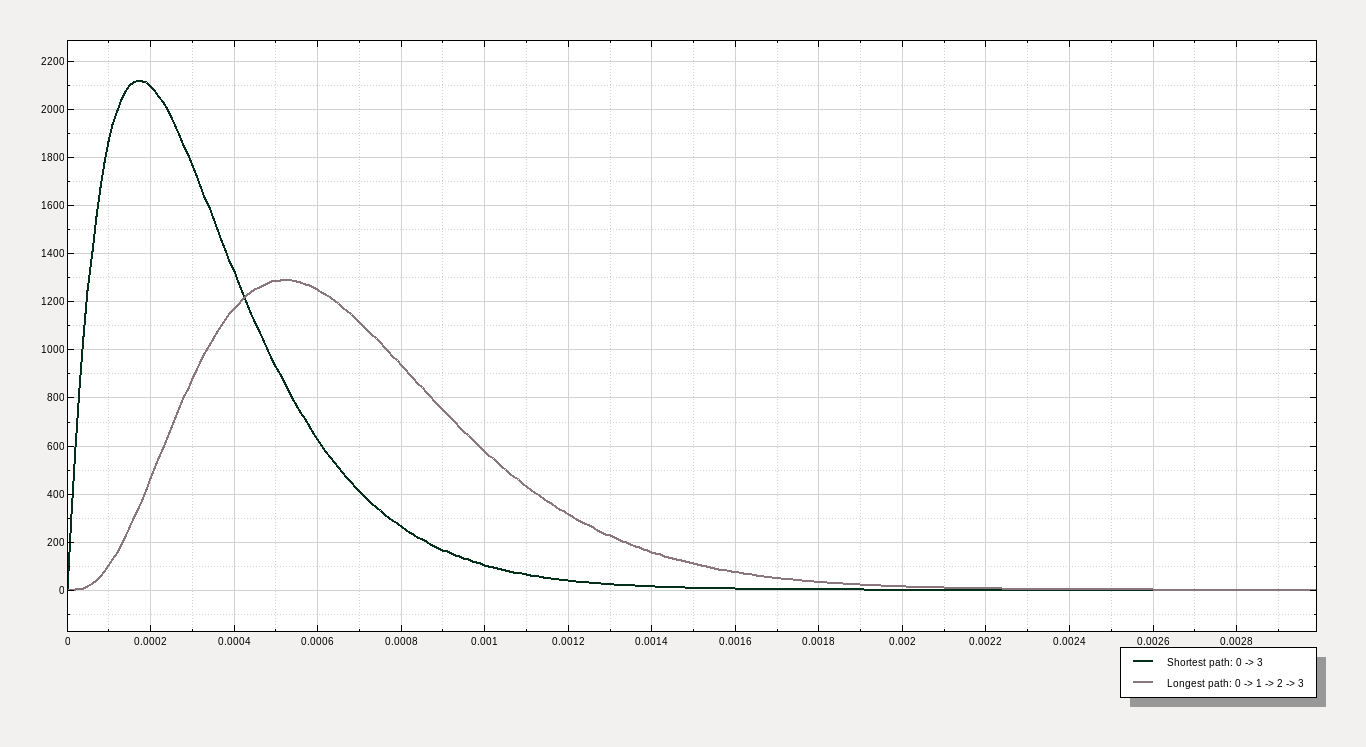
\includegraphics[width=\textwidth]{demo4_chart}
	
	\caption{Графики плотностей распределения количества сообщений в самом коротком и самом длинном маршрутах сети}
	\label{pic:demo4_graph}
\end{figure}

% ------------------------------------ code ------------------------------------
\begin{figure}[h!]
    \begin{listing}{1}
void ComputeParameters()
{
  // вычисление суммарной интенсивности внешних потоков
  Lambda.ForEach(
	lambdas => Lambda0.AddElement(lambdas.Sum())); 
  RoTotal = new Vector<double>(NodesCount);

  for (int stream = 0; stream < StreamsCount; stream++)
  {
	// вычисление входных вероятностей
	InputProbability.Add(Lambda[stream].Clone()
	  .InsertElement(0, 0).Divide(Lambda0[stream]));
	// вычисление коэфициентов передачи
	E.Add(
	  GaussMethod.Solve(GetExtendedMatrix(stream)));
	// вычисление общих интенсивностей потоков
	LambdaBar.Add(
	  E[stream].Multiply(Lambda0[stream]));
	// вычисление коэффициентов использования узлов
	RoBar.Add(
	  LambdaBar[stream].DivideElementWise(Mu[stream]));
	RoTotal = RoTotal.AddElementWise(RoBar.Last());
	
  	if(RoBar[stream].Any(roBar => roBar > 1))
	  throw new ArgumentOutOfRangeException(
	  string.Format("RoBar, stream {0}", stream),
	  "Some Ro' is greater than zero.");
  }
  if (RoTotal.Any(roTotal => roTotal > 1))
	throw new ArgumentOutOfRangeException("RoTotal",
	"Some RoTotal is greater than zero.");
	
	FindPaths();
}\end{listing}
	
	\caption{Функция расчёта параметров модели}
	\label{pic:function_computeParameters}
\end{figure}

\begin{figure}[h!]
    \begin{listing}{1}
Matrix<double> GetExtendedMatrix(int streamIndex)
{
  var matrix = GetRoutingMatrix(streamIndex);
  matrix.Transpose();
  matrix.RemoveRow(0);
  matrix.AddColumn(matrix.GetColumn(0).Negate());
  matrix.RemoveColumn(0);
  matrix.ReplaceDiagonalElements(-1);

  return matrix;
}\end{listing}
    
    \caption{Функция преобразования мартрицы маршрутизации в расширенную матрицу системы уравнений баланса}
    \label{pic:functions_getextendedmatrix}
\end{figure}

\begin{figure}[h!]
	\begin{listing}{1}
void ComputeStationaryPTC()
{
  for (int i = 0; i < NodesCount; i++)
  {
	double sum = 0.0;
	for (int stream = 0; stream < StreamsCount; stream++)
	  sum += RoBar[stream][i] / Mu[stream][i];

	Ws.AddElement(sum / (1 - RoTotal[i]));
  }

  for (int stream = 0; stream < StreamsCount; stream++)
  {
	Us.Add( Ws.AddElementWise(Mu[stream].Pow(-1)) );
	Ls.Add(
	  LambdaBar[stream].MultiplyElementWise(Ws) );
	Ns.Add(
	  LambdaBar[stream].MultiplyElementWise(Us[stream]));
  }
}\end{listing}

	\caption{Функция вычисления стационарных ВВХ}
	\label{pic:function_computeSPTC}
\end{figure}

\begin{figure}[h!]
	\begin{listing}{1}
void ComputeIntegratedPTC()
{
  ComputeTransitionProbabilities();

  Wi = ComputeIntegralChar(Ws);
  for (int stream = 0; stream < StreamsCount; stream++)
  {
	Ui.Add(ComputeIntegralChar(Us[stream]));
	Li.Add(ComputeIntegralChar(Ls[stream]));
	Ni.Add(ComputeIntegralChar(Ns[stream]));
  }
}\end{listing}

	\caption{Функция вычисления интегральных ВВХ}
	\label{pic:function_computeIPTC}
\end{figure}

\begin{figure}[h!]
	\begin{listing}{1}
double ComputeIntegralChar(Vector<double> staticChar)
{
  var integralChar =
	staticChar[StartNode] + staticChar[TargetNode];

  for (int i = 0; i < Paths.Count(); i++)
  {
	var temp = 0.0;
	for (int j=1; j < Paths.ElementAt(i).Count()-1; j++)
	  temp += staticChar[j];

	integralChar += TransitionProbabilities[i] * temp;
  }

  return integralChar;
}\end{listing}

	\caption{}
	\label{pic:function_computeIntegralChar}
\end{figure}

\begin{figure}[h!]
	\begin{listing}{1}
void ComputeTransitionProbabilities()
  {
	var matrix = RoutingMatrix.Clone().RemoveColumn(0);

	var pathsProbabilities = 
	Paths.Select(
	path => path.Where(
	(item, index) => index < path.Length - 1)
	.Select((item, index) => new {item, index})
	.Aggregate(1.0, (accumulate, anon) => accumulate *=
	matrix[anon.item, path[anon.index + 1]]));

	var s = pathsProbabilities.Sum();

	TransitionProbabilities = pathsProbabilities
	.Select(prob => prob / s).ToList();
}\end{listing}

	\caption{Функция вычисления вероятностей выбора маршрутов}
	\label{pic:function_computeTransitionProbabilities}
\end{figure}

\begin{figure}[h!]
	\begin{listing}{1}
List<Vector<int>> GetPathsBetween(
  Matrix<double> matrix, int startNode, int targetNode)
{
  if (startNode == targetNode)
  throw new ArgumentException(
  "stratNode and targetNode must be different.");

  var paths = new List<Vector<int>>();

  // исключение циклов
  matrix.ForEachRow(row => row[startNode] = 0);

  for (int intermediateNode = 0;
  intermediateNode < matrix.RowsCount; intermediateNode++)
  {
	if (matrix[startNode, intermediateNode] <= 0)
	  continue;

	if (intermediateNode == targetNode)
	  paths.Add(
	  new Vector<int>(new[] { startNode, targetNode }));
	else
	{
	  List<Vector<int>> localPaths = GetPathsBetween(
	  matrix.Clone(), intermediateNode, targetNode);
	  if (localPaths.Any())
		localPaths.ForEach(path =>
	  	{
		  path.InsertElement(0, startNode);
		  paths.Add(path);
	  	});
	  }
    }

  return paths;
}\end{listing}

	\caption{Функция поиска всех путей между двумя вершинами}
	\label{pic:function_getPathsBetween}
\end{figure}

\begin{figure}[h!]
	\begin{listing}{1}
void FindPaths()
{
  var matrix = RoutingMatrix.Clone().RemoveColumn(0);
  var pathsCount = 0;
  var pairsCount = 0;

  for (int startNode = 0; startNode < matrix.RowsCount;
  	startNode++)
	for (int targetNode = 0;
	targetNode < matrix.RowsCount;targetNode++)
	  if (startNode != targetNode)
	  {	
		var paths = GraphHelper.GetPathsBetween(
		  matrix.Clone(), startNode, targetNode);

		if (startNode == StartNode
		  && targetNode == TargetNode)
		    Paths = paths;

		pathsCount += paths.Count();
		pairsCount++;							

		if (MinPath == null
		  || paths.Min().Length < MinPath.Length)
		    MinPath = paths.Min();
		if (MaxPath == null
		  || paths.Max().Length > MaxPath.Length)
		    MaxPath = paths.Max();
	  }

  AveragePaths = pathsCount / pairsCount;
}\end{listing}

	\caption{Функция поиска путей, минамального и максимального пути, среднее количество путей}
	\label{pic:function_findPaths}
\end{figure}

\begin{figure}[h!]
	\begin{listing}{1}
NAME = Full-mesh topology
STREAMS COUNT = 2
==================== STREAM 0 ====================
ROUTING MATRIX
0.000	0.271	0.293	0.211	0.224
0.250	0.000	0.250	0.250	0.250
0.250	0.250	0.000	0.250	0.250
0.250	0.250	0.250	0.000	0.250
0.250	0.250	0.250	0.250	0.000

LAMBDA
860.000000
930.000000
670.000000
710.000000

MU
8928.571429
8928.571429
8928.571429
8928.571429

RO
0.096320
0.104160
0.075040
0.079520

LAMBDA0
3170

E
1.017035
1.034700
0.969085
0.979180

LAMBDA'
3224.000000
3280.000000
3072.000000
3104.000000\end{listing}

	\label{pic:demo4_log_begin}
\end{figure}

\begin{figure}[h!]
	\begin{listing}{43}
RO'
0.361088
0.367360
0.344064
0.347648

ROTOTAL
0.899476
0.900444
0.888420
0.890015

THE AVERAGE NUMBER OF PATHS
5.000000

STATIONARY PROBABILITY-TIME CHARACTERISTICS
W
0.004841
0.004851
0.004389
0.004441

U
0.004953
0.004963
0.004501
0.004553

L
15.608149
15.911909
13.482236
13.785019

N
15.969237
16.279269
13.826300
14.132667\end{listing}
\end{figure}

\begin{figure}[h!]
	\begin{listing}{82}
INTEGRATED PROBABILITY-TIME CHARACTERISTICS
PATHS, 5
0 -> 3 : 0.615384615384615
0 -> 1 -> 3 : 0.153846153846154
0 -> 2 -> 3 : 0.153846153846154
0 -> 1 -> 2 -> 3 : 0.0384615384615385
0 -> 2 -> 1 -> 3 : 0.0384615384615385

W
0.011486

U
0.011761

L
36.550228

N
37.426723
==================================================

==================== STREAM 1 ====================
ROUTING MATRIX
0.000	0.247	0.235	0.261	0.257
0.250	0.000	0.250	0.250	0.250
0.250	0.250	0.000	0.250	0.250
0.250	0.250	0.250	0.000	0.250
0.250	0.250	0.250	0.250	0.000

LAMBDA
161.000000
153.000000
170.000000
167.000000

MU
1206.563707
1206.563707
1206.563707
1206.563707\end{listing}
\end{figure}

\begin{figure}[h!]
	\begin{listing}{122}
RO
0.133437
0.126806
0.140896
0.138410

LAMBDA0
651

E
0.997849
0.988018
1.008909
1.005223

LAMBDA'
649.600000
643.200000
656.800000
654.400000

RO'
0.538388
0.533084
0.544356
0.542367

ROTOTAL
0.899476
0.900444
0.888420
0.890015

THE AVERAGE NUMBER OF PATHS
5.000000

STATIONARY PROBABILITY-TIME CHARACTERISTICS
W
0.004841
0.004851
0.004389
0.004441\end{listing}
\end{figure}

\begin{figure}[h!]
	\begin{listing}{164}
U
0.005670
0.005680
0.005218
0.005270

L
3.144868
3.120287
2.882530
2.906223

N
3.683256
3.653371
3.426886
3.448590

INTEGRATED PROBABILITY-TIME CHARACTERISTICS
PATHS, 5
0 -> 3 : 0.615384615384615
0 -> 1 -> 3 : 0.153846153846154
0 -> 2 -> 3 : 0.153846153846154
0 -> 1 -> 2 -> 3 : 0.0384615384615385
0 -> 2 -> 1 -> 3 : 0.0384615384615385

W
0.011486

U
0.013526

L
7.472934

N
8.800595
==================================================\end{listing}

	\caption{Лог для полносвязной сети из 4-х узлов с двумя потоками}
	\label{pic:demo4_log_end}
\end{figure}
% ------------------------------------------------------------------------------

\Chapter{Модельный эксперимент}
\Section{Задачи}
В задачи проведения модельного эксперимента входит сравнение разных топологий сетей по характеристикам времени и надёжности доставки сообщений, определение топологий с самым малым временем доставки сообщений и самой большой надёжностью доставки.

\Section{Методология}
Для качетсвенного проведения эксперимента надо исключить любые факторы, которые могут повлиять на его ход и результаты. В данном случае, для сравнения именно топологий сетей и как они влияют на храктеристики времени и надёжности доставки сообщений, будем сравнивать сети с одним потоком сообщений, с одинаковым количеством узлом, одинаковыми интенсивностями внешних источников и одинаковыми интенсивностями обработки собщений. У всех сравниваемых моделей будет отличаться только структура связей между узлами.

Для определения самой эффективной по времени доставки топологии, сети будем использовать интегральную вероятностно-временную характеристику \( U \) (\ref{subsection:iptc}), характеризующей среднее время пребывания требования в маршруте.

Для определения топологии, предоставляющей самую надёжную доставку сообщений, будем сравнивать сети по среднему числу путей между любыми двумя узлами сети.

Для этого эксперимента будем использовать модели сетей с 10 узлами, интенсивностью обработки сообщений соответствующей технологии 10G Ethernet с кадрами максимальной длины, интенсивностью поступления сообщений из внешнего источника равной 7\% (5.689207 сообщений/мс) от интенсивности обработки и следующими топологиями:
\begin{enumerate}
	\item Шина	
	\item Звезда
	\item Кольцо
	\item Дерево
	\item Двухменая квадратная решётка
	\item Двухмерная треугольная решётка
	\item Трёхмерная квадратная решётся
	\item Пирамидальная топология	
	\item Полносвязная топология
\end{enumerate}

\Section{Анализ полученных данных}
В результате моделирования получены данные, приведённые в таблице \ref{tab:modeling_result}. Из них видно, что от топологии сети зависит многое. При одинаковом числе узлов, входных интенсивностях и интенсивностях обработки сообщений, различные топологии дают совешенно различные результаты по скорости и надёжности доставки сообщений.

У базовых топологий (шина, звезда, кольцо и дерево) самое минимальное возможное среднее число путей, что делает их совершенно не устойчивым к отказам. Шина также имеет самое большое время доставки.

Полносвязная топология самая надёжная с средним числом путей между любыми двумя вершинами 109601, но время доставки сообщений в ней не лучшее.

Топологией с самой быстрой доставкой сообещений (0.008404 мс)  --- \\ пирамидальная топология.

Пирамидальная топология лучшая по скорости доставки сообщений и вторая по надёжности, а полносвязная лучшая по надёжности и вторая по скорости доставки.

Также можно сравнить топологии по количеству связей, образующих их.

Топологии шина, звезда, кольцо и дерево имеют минимальное необходимое количество связей для сооединения 10-ти узлов. Именно из-за отсутствия избыточности эти топологии имееют самую низкую надёжность.

Если сравнивать полносвязную и пирамидальную топологии по числу связей, то у полносвязной их \( \frac{ n * (n - 1) }{2} = \frac{10 * 9}{2} = 45 \), а у пирамидальной 24, что в 1.875 раза меньше. С этой точки зрения пирамидальная топология выглядит привлекательнее полносвязной, потому что при почти в два раза меньшем количестве связей эта топология имеет лучшее время доставки и второй показатель надёжности.

У двухмерной квадратной решётки, как и у пирамидальной, 24 связи, но хуже время доставки и малое среднее число путей между любыми двумя узлами. 

Двухмерная треугольная и трёхмерная квадратная решётки имеют хорошее соотношение между временем доставки, надёжностью и количеством связей.

\begin{table}[h!]
	\begin{tabular}{|p{0.22\textwidth}|p{0.22\textwidth}|p{0.22\textwidth}|p{0.22\textwidth}|}
	\hline Топология & Среднее время пребывания требования в маршруте (мс) & Среднее число путей между любыми двумя узлами & Количество связей \\
	\hline Шина  & 0.153211 & 1 & 9 \\
	\hline Звезда & 0.055320 & 1 & 9 \\
	\hline Кольцо & 0.014307 & 1 & 10 \\
	\hline Дерево & 0.064059 & 1 & 9 \\
	\hline Двухменая квадратная решётка & 0.082925 & 4.844444 & 24 \\
	\hline Двухмерная треугольная решётка & 0.089373 & 50.733333 & 18 \\
	\hline Трёхмерная квадратная решётся & 0.069486 & 24.2 & 15 \\
	\hline Пирамидальная топология & 0.008404 & 503.522222 & 24 \\
	\hline Полносвязная топология & 0.013876 & 109601 & 45 \\
	\hline
	\end{tabular}
	
	\caption{Результаты модельного эксперимента}
	\label{tab:modeling_result}
\end{table}

\chapter*{\centering Заключение}
\addcontentsline{toc}{chapter}{Заключение}
В дипломной работе выполнено следующее:	
\begin{enumerate}
	\item Изучена методика построения моеделей информационно- \\ вычислительных сетей.
	 
	\item Разработанна программа, автоматизирующая вычисления стационарных и интегральных вероятностно-временных характеристик, плотностей распределения сообщений в маршрутах сети и среднего количества маршрутов между любыми двумя узлами сети на основе заданной модели сети.
	Она будет полезна при:
	\begin{itemize}
		\item[-] предварительной оценке характеристик проектируемой ИВС
		\item[-] оценке характеристик уже существующих ИВС
		\item[-] изучении влияния изменений топологии и/или оборудования на характеристики ИВС
	\end{itemize}
	
	\item Корректность работы программы и адекватность результатов проверена на моделях из \cite{klimanov:manual_stankin}.
	
	\item Разработаны модели сетей с раными топологиями и с помощью разработанной программы проведён модельный эксперимент по их сравнению по времени и надёжности доставки сообщений.
\end{enumerate}

Планирую дальнейшее развитие разработанной программы, улучшение функционала и производительности, поддержка различных методов аналитического моделирования для разных моделей сетей.

\renewcommand{\bibname}{\centering Список литературы}
\begin{thebibliography}{00}
\addcontentsline{toc}{chapter}{Список литературы}

\bibitem{vishnevsky} Вишневский В.М.
Теоретические основы проектирования компьютерных сетей: монография.
--- Москва: Техносфера, 2003.
--- 512 с.

\bibitem{kleinrock} Клейнрок Л.
Теория массового обслуживания.
--- Москва: Машиностроение, 1979.
--- 432 с.

\bibitem{klimanov:thesis} Климанов В.П.
Методология анализа вероятностно-временных характеристик локальных вычислительных сетей составных топологий на основе аналитического
моделирования: автореферат диссертации на соискание учёной степени доктора технических наук.
--- Москва: Московский энергетический институт, 1993.
--- 40 с.

\bibitem{klimanov:manual_mpei} Климанов В.П.
Методы разработки аналитических моделей для анализа локальных вычислительных сетей, используемых в управлении технологическим процессом: учебное пособие
--- Москва: Московский энергетический институт, 1995.
--- 115 с.

\bibitem{klimanov:manual_stankin} Климанов В.П., Руделёв Р.А.
Моделирование информационных систем. Математические модели для разработки информационных систем: методика и решения: учебное пособие.
--- Москва: ФГБОУ ВПО МГТУ <<СТАНКИН>>, 2014.
--- 45 с.

\bibitem{olifers} Олифер В.Г., Олифер Н.А.
Компьютерные сети. Принципы, технологии, протоколы: учебник для вузов.
--- 4-е изд.
--- Санкт-Петербург: Питер, 2010.
--- 944 с.

\bibitem{pisarev} Писарев В.Н.
Применение теории массового обслуживания в задачах инженерно-авиационного обеспечения.
--- Типография ВВИА имени проф. Н.Е. ~Жукова, 1965.
--- 45 с.

\bibitem{hinchin} Хинчин А.Я.
Работы по математической теории массового обслуживания
--- Москва: Физматгиз, 1963.
--- 236 с.

\bibitem{reliability}
Файловый архив для студентов.
--- [Электронный ресурс]. Дата обновления: 11.04.2015.
--- URL: http://www.studfiles.ru/preview/2948129/ (дата обращения: 06.06.2015).

\end{thebibliography}
\end{document}